\documentclass{standalone}
\usepackage{tikz}
\usetikzlibrary{patterns, positioning}
\usepackage[sfdefault]{ClearSans} %% option 'sfdefault' activates Clear Sans as the default text font
\usepackage[T1]{fontenc}

\begin{document}
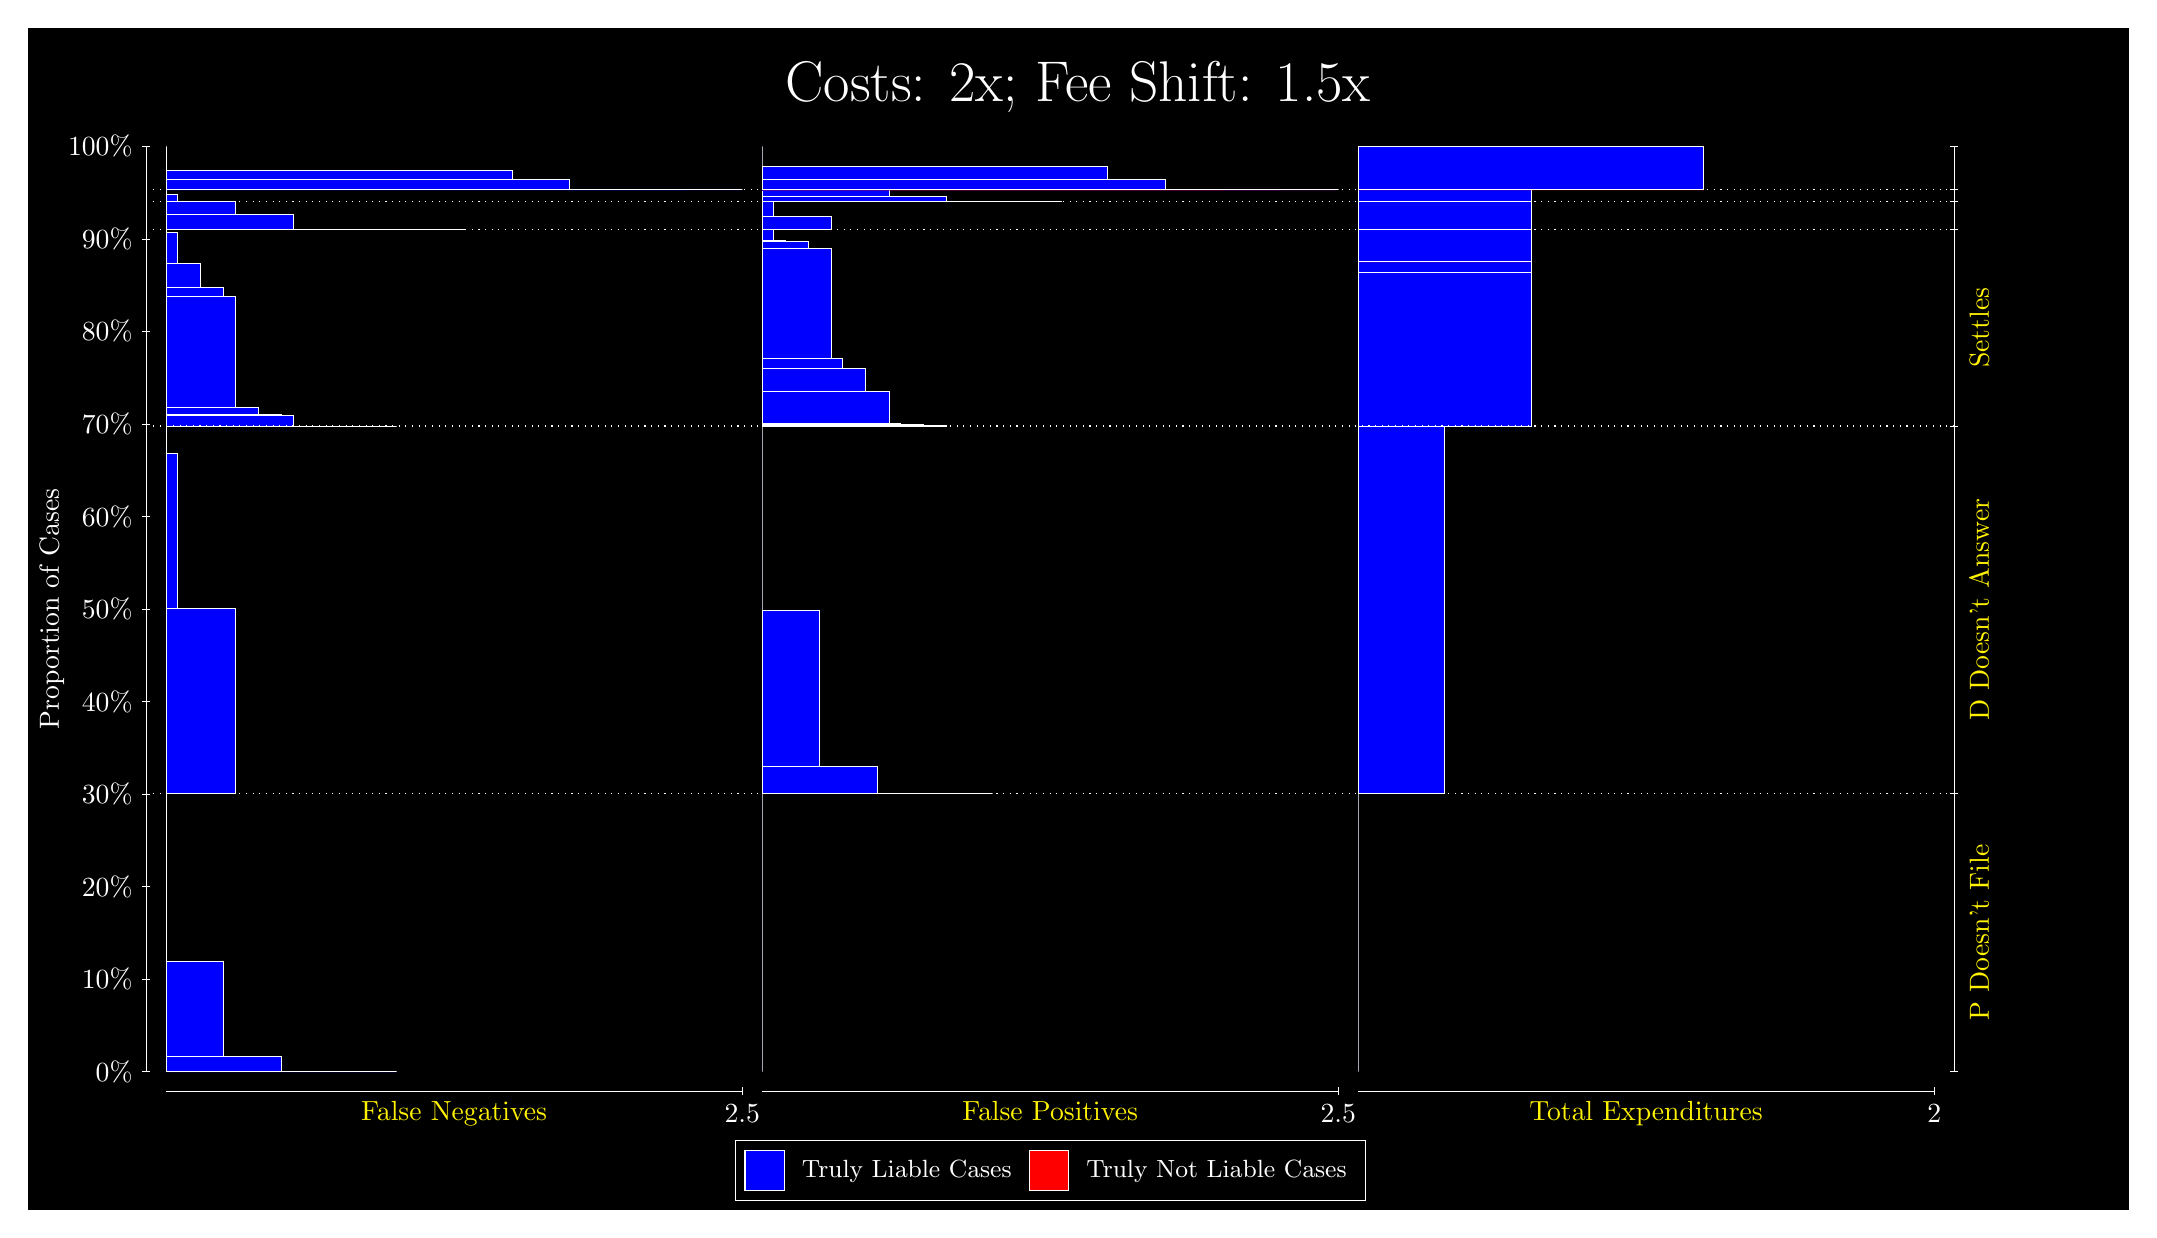
\begin{tikzpicture}
\draw[fill=black] (0,0) rectangle (26.667,15);
\draw[text=white] (0,13.5) rectangle (26.667,15) node[midway] {\huge Costs: 2x; Fee Shift: 1.5x};
\draw[white, very thin] (1.5,1.75) -- (1.5,13.5);
\node[rotate=90, text=white, anchor=center] at (0.3, 7.625) {Proportion of Cases};
\draw[white, very thin] (1.45,1.75) -- (1.55,1.75);
\node[text=white, anchor=east] at (1.45, 1.75) {0\%};
\draw[white, very thin] (1.45,2.925) -- (1.55,2.925);
\node[text=white, anchor=east] at (1.45, 2.925) {10\%};
\draw[white, very thin] (1.45,4.1) -- (1.55,4.1);
\node[text=white, anchor=east] at (1.45, 4.1) {20\%};
\draw[white, very thin] (1.45,5.275) -- (1.55,5.275);
\node[text=white, anchor=east] at (1.45, 5.275) {30\%};
\draw[white, very thin] (1.45,6.45) -- (1.55,6.45);
\node[text=white, anchor=east] at (1.45, 6.45) {40\%};
\draw[white, very thin] (1.45,7.625) -- (1.55,7.625);
\node[text=white, anchor=east] at (1.45, 7.625) {50\%};
\draw[white, very thin] (1.45,8.8) -- (1.55,8.8);
\node[text=white, anchor=east] at (1.45, 8.8) {60\%};
\draw[white, very thin] (1.45,9.975) -- (1.55,9.975);
\node[text=white, anchor=east] at (1.45, 9.975) {70\%};
\draw[white, very thin] (1.45,11.15) -- (1.55,11.15);
\node[text=white, anchor=east] at (1.45, 11.15) {80\%};
\draw[white, very thin] (1.45,12.325) -- (1.55,12.325);
\node[text=white, anchor=east] at (1.45, 12.325) {90\%};
\draw[white, very thin] (1.45,13.5) -- (1.55,13.5);
\node[text=white, anchor=east] at (1.45, 13.5) {100\%};

\draw[white, very thin] (24.457,1.75) -- (24.457,13.5);
\draw[white, very thin] (24.407,1.75) -- (24.507,1.75);
\node[anchor=west] at (24.407, 1.75) {};
\draw[white, very thin] (24.407,5.2838) -- (24.507,5.2838);
\node[anchor=west] at (24.407, 5.2838) {};
\draw[white, very thin] (24.407,9.9488) -- (24.507,9.9488);
\node[anchor=west] at (24.407, 9.9488) {};
\draw[white, very thin] (24.407,12.444) -- (24.507,12.444);
\node[anchor=west] at (24.407, 12.444) {};
\draw[white, very thin] (24.407,12.804) -- (24.507,12.804);
\node[anchor=west] at (24.407, 12.804) {};
\draw[white, very thin] (24.407,12.95) -- (24.507,12.95);
\node[anchor=west] at (24.407, 12.95) {};
\draw[white, very thin] (24.407,13.5) -- (24.507,13.5);
\node[anchor=west] at (24.407, 13.5) {};

\draw[white, very thin, fill=blue] (1.75,1.75) rectangle (4.6775,1.75);
\draw[white, very thin, fill=blue] (1.75,1.75) rectangle (3.9457,1.7516);
\draw[white, very thin, fill=blue] (1.75,1.7516) rectangle (3.2138,1.9464);
\draw[white, very thin, fill=blue] (1.75,1.9464) rectangle (2.4819,3.1492);
\draw[white, very thin, fill=red] (1.75,3.1492) rectangle (1.75,3.1492);
\draw[white, very thin, fill=blue] (1.75,3.1492) rectangle (1.75,5.2838);
\draw[white, very thin, fill=blue] (1.75,5.2838) rectangle (2.6283,7.63);
\draw[white, very thin, fill=blue] (1.75,7.63) rectangle (1.8964,9.6053);
\draw[white, very thin, fill=red] (1.75,9.6053) rectangle (1.75,9.6053);
\draw[white, very thin, fill=blue] (1.75,9.6053) rectangle (1.75,9.9488);
\draw[white, very thin, fill=blue] (1.75,9.9488) rectangle (4.6775,9.9488);
\draw[white, very thin, fill=blue] (1.75,9.9488) rectangle (4.3848,9.9488);
\draw[white, very thin, fill=blue] (1.75,9.9488) rectangle (4.092,9.949);
\draw[white, very thin, fill=blue] (1.75,9.949) rectangle (3.9457,9.949);
\draw[white, very thin, fill=blue] (1.75,9.949) rectangle (3.6529,9.9492);
\draw[white, very thin, fill=blue] (1.75,9.9492) rectangle (3.3602,10.089);
\draw[white, very thin, fill=blue] (1.75,10.089) rectangle (3.2138,10.095);
\draw[white, very thin, fill=blue] (1.75,10.095) rectangle (2.921,10.185);
\draw[white, very thin, fill=blue] (1.75,10.185) rectangle (2.6283,11.59);
\draw[white, very thin, fill=blue] (1.75,11.59) rectangle (2.4819,11.707);
\draw[white, very thin, fill=blue] (1.75,11.707) rectangle (2.1891,12.009);
\draw[white, very thin, fill=blue] (1.75,12.009) rectangle (1.8964,12.404);
\draw[white, very thin, fill=red] (1.75,12.404) rectangle (1.75,12.404);
\draw[white, very thin, fill=blue] (1.75,12.404) rectangle (1.75,12.444);
\draw[white, very thin, fill=blue] (1.75,12.444) rectangle (5.5558,12.444);
\draw[white, very thin, fill=blue] (1.75,12.444) rectangle (4.8239,12.444);
\draw[white, very thin, fill=blue] (1.75,12.444) rectangle (4.092,12.447);
\draw[white, very thin, fill=blue] (1.75,12.447) rectangle (3.3602,12.631);
\draw[white, very thin, fill=blue] (1.75,12.631) rectangle (2.6283,12.804);
\draw[white, very thin, fill=red] (1.75,12.804) rectangle (1.75,12.804);
\draw[white, very thin, fill=blue] (1.75,12.804) rectangle (2.6283,12.806);
\draw[white, very thin, fill=blue] (1.75,12.806) rectangle (1.8964,12.888);
\draw[white, very thin, fill=red] (1.75,12.888) rectangle (1.75,12.888);
\draw[white, very thin, fill=blue] (1.75,12.888) rectangle (1.75,12.95);
\draw[white, very thin, fill=blue] (1.75,12.95) rectangle (9.0689,12.95);
\draw[white, very thin, fill=blue] (1.75,12.95) rectangle (8.337,12.95);
\draw[white, very thin, fill=blue] (1.75,12.95) rectangle (7.6051,12.959);
\draw[white, very thin, fill=blue] (1.75,12.959) rectangle (6.8732,13.085);
\draw[white, very thin, fill=blue] (1.75,13.085) rectangle (6.1413,13.201);
\draw[white, very thin, fill=blue] (1.75,13.201) rectangle (5.4094,13.202);
\draw[white, very thin, fill=blue] (1.75,13.202) rectangle (4.6775,13.202);
\draw[white, very thin, fill=blue] (1.75,13.202) rectangle (3.0674,13.202);
\draw[white, very thin, fill=blue] (1.75,13.202) rectangle (2.3355,13.202);
\draw[white, very thin, fill=red] (1.75,13.202) rectangle (1.75,13.202);
\draw[white, very thin, fill=blue] (1.75,13.202) rectangle (1.75,13.5);
\draw[white, very thin, fill=red] (9.3189,1.75) rectangle (9.3189,1.75);
\draw[white, very thin, fill=blue] (9.3189,1.75) rectangle (9.3189,5.2838);
\draw[white, very thin, fill=red] (9.3189,5.2838) rectangle (12.246,5.2838);
\draw[white, very thin, fill=blue] (9.3189,5.2838) rectangle (12.246,5.2838);
\draw[white, very thin, fill=blue] (9.3189,5.2838) rectangle (11.515,5.2854);
\draw[white, very thin, fill=blue] (9.3189,5.2854) rectangle (10.783,5.6273);
\draw[white, very thin, fill=blue] (9.3189,5.6273) rectangle (10.051,7.6026);
\draw[white, very thin, fill=blue] (9.3189,7.6026) rectangle (9.3189,9.9488);
\draw[white, very thin, fill=red] (9.3189,9.9488) rectangle (11.661,9.9488);
\draw[white, very thin, fill=blue] (9.3189,9.9488) rectangle (11.661,9.9588);
\draw[white, very thin, fill=red] (9.3189,9.9588) rectangle (11.368,9.9588);
\draw[white, very thin, fill=blue] (9.3189,9.9588) rectangle (11.368,9.9757);
\draw[white, very thin, fill=red] (9.3189,9.9757) rectangle (11.075,9.9757);
\draw[white, very thin, fill=blue] (9.3189,9.9757) rectangle (11.075,9.988);
\draw[white, very thin, fill=blue] (9.3189,9.988) rectangle (10.929,10.384);
\draw[white, very thin, fill=blue] (9.3189,10.384) rectangle (10.636,10.685);
\draw[white, very thin, fill=blue] (9.3189,10.685) rectangle (10.344,10.803);
\draw[white, very thin, fill=blue] (9.3189,10.803) rectangle (10.197,12.208);
\draw[white, very thin, fill=blue] (9.3189,12.208) rectangle (9.9044,12.297);
\draw[white, very thin, fill=blue] (9.3189,12.297) rectangle (9.6116,12.303);
\draw[white, very thin, fill=blue] (9.3189,12.303) rectangle (9.4652,12.443);
\draw[white, very thin, fill=blue] (9.3189,12.443) rectangle (9.3189,12.444);
\draw[white, very thin, fill=red] (9.3189,12.444) rectangle (10.197,12.444);
\draw[white, very thin, fill=blue] (9.3189,12.444) rectangle (10.197,12.617);
\draw[white, very thin, fill=blue] (9.3189,12.617) rectangle (9.4652,12.801);
\draw[white, very thin, fill=blue] (9.3189,12.801) rectangle (9.3189,12.804);
\draw[white, very thin, fill=red] (9.3189,12.804) rectangle (13.125,12.804);
\draw[white, very thin, fill=blue] (9.3189,12.804) rectangle (13.125,12.804);
\draw[white, very thin, fill=blue] (9.3189,12.804) rectangle (12.393,12.804);
\draw[white, very thin, fill=blue] (9.3189,12.804) rectangle (11.661,12.867);
\draw[white, very thin, fill=blue] (9.3189,12.867) rectangle (10.929,12.949);
\draw[white, very thin, fill=blue] (9.3189,12.949) rectangle (10.197,12.95);
\draw[white, very thin, fill=red] (9.3189,12.95) rectangle (16.638,12.95);
\draw[white, very thin, fill=blue] (9.3189,12.95) rectangle (16.638,12.95);
\draw[white, very thin, fill=red] (9.3189,12.95) rectangle (15.906,12.95);
\draw[white, very thin, fill=blue] (9.3189,12.95) rectangle (15.906,12.95);
\draw[white, very thin, fill=red] (9.3189,12.95) rectangle (15.174,12.95);
\draw[white, very thin, fill=blue] (9.3189,12.95) rectangle (15.174,12.959);
\draw[white, very thin, fill=red] (9.3189,12.959) rectangle (14.442,12.959);
\draw[white, very thin, fill=blue] (9.3189,12.959) rectangle (14.442,13.086);
\draw[white, very thin, fill=blue] (9.3189,13.086) rectangle (13.71,13.247);
\draw[white, very thin, fill=blue] (9.3189,13.247) rectangle (12.978,13.248);
\draw[white, very thin, fill=blue] (9.3189,13.248) rectangle (12.246,13.248);
\draw[white, very thin, fill=blue] (9.3189,13.248) rectangle (11.515,13.248);
\draw[white, very thin, fill=red] (9.3189,13.248) rectangle (9.9044,13.248);
\draw[white, very thin, fill=blue] (9.3189,13.248) rectangle (9.9044,13.248);
\draw[white, very thin, fill=red] (9.3189,13.248) rectangle (9.3189,13.248);
\draw[white, very thin, fill=blue] (9.3189,13.248) rectangle (9.3189,13.5);
\draw[white, very thin, fill=red] (16.888,1.75) rectangle (16.888,1.75);
\draw[white, very thin, fill=blue] (16.888,1.75) rectangle (16.888,5.2838);
\draw[white, very thin, fill=red] (16.888,5.2838) rectangle (17.986,5.2838);
\draw[white, very thin, fill=blue] (16.888,5.2838) rectangle (17.986,9.9488);
\draw[white, very thin, fill=red] (16.888,9.9488) rectangle (19.083,9.9488);
\draw[white, very thin, fill=blue] (16.888,9.9488) rectangle (19.083,11.899);
\draw[white, very thin, fill=red] (16.888,11.899) rectangle (19.083,11.899);
\draw[white, very thin, fill=blue] (16.888,11.899) rectangle (19.083,12.036);
\draw[white, very thin, fill=red] (16.888,12.036) rectangle (19.083,12.036);
\draw[white, very thin, fill=blue] (16.888,12.036) rectangle (19.083,12.444);
\draw[white, very thin, fill=red] (16.888,12.444) rectangle (19.083,12.444);
\draw[white, very thin, fill=blue] (16.888,12.444) rectangle (19.083,12.804);
\draw[white, very thin, fill=red] (16.888,12.804) rectangle (19.083,12.804);
\draw[white, very thin, fill=blue] (16.888,12.804) rectangle (19.083,12.95);
\draw[white, very thin, fill=red] (16.888,12.95) rectangle (21.279,12.95);
\draw[white, very thin, fill=blue] (16.888,12.95) rectangle (21.279,13.5);
\draw[white, dotted] (1.5,5.2838) -- (24.457,5.2838);
\draw[white, dotted] (1.5,9.9488) -- (24.457,9.9488);
\draw[white, dotted] (1.5,12.444) -- (24.457,12.444);
\draw[white, dotted] (1.5,12.804) -- (24.457,12.804);
\draw[white, dotted] (1.5,12.95) -- (24.457,12.95);
\draw[white, very thin] (1.75,1.5) -- (9.0689,1.5);
\node[text=yellow, anchor=north] at (5.4094, 1.5) {False Negatives};
\draw[white, very thin] (9.0689,1.45) -- (9.0689,1.55);
\node[text=white, anchor=north] at (9.0689, 1.45) {2.5};

\draw[white, very thin] (9.3189,1.5) -- (16.638,1.5);
\node[text=yellow, anchor=north] at (12.978, 1.5) {False Positives};
\draw[white, very thin] (16.638,1.45) -- (16.638,1.55);
\node[text=white, anchor=north] at (16.638, 1.45) {2.5};

\draw[white, very thin] (16.888,1.5) -- (24.207,1.5);
\node[text=yellow, anchor=north] at (20.547, 1.5) {Total Expenditures};
\draw[white, very thin] (24.207,1.45) -- (24.207,1.55);
\node[text=white, anchor=north] at (24.207, 1.45) {2};

\node[text=yellow, centered, rotate=90] at (24.777, 3.5169) {P Doesn't File};
\node[text=yellow, centered, rotate=90] at (24.777, 7.6163) {D Doesn't Answer};
\node[text=yellow, centered, rotate=90] at (24.777, 11.196) {Settles};




\draw (12.978300999999998,1.5) node[draw=none] (baseCoordinate) {};
\begin{scope}[align=center]
        \matrix[scale=0.5, draw=white, below=0.5cm of baseCoordinate, nodes={draw}, column sep=0.1cm]{
            \node[rectangle, draw, minimum width=0.5cm, minimum height=0.5cm, fill=blue] {}; &
            \node[draw=none, font=\small, text=white] (B) {Truly Liable Cases}; &
            \node[rectangle, draw, minimum width=0.5cm, minimum height=0.5cm, fill=red] {}; &
            \node[draw=none, font=\small, text=white] (B) {Truly Not Liable Cases}; \\
            };
\end{scope}

\end{tikzpicture}
\end{document}